\documentclass[12pt, a4paper]{article}

\usepackage[utf8]{inputenc}
\usepackage[T1]{fontenc}
\usepackage[spanish]{babel}
\usepackage{amsmath, amssymb}
\usepackage{geometry}
\usepackage{graphicx}
\usepackage{float}
\usepackage{booktabs}
\usepackage{hyperref}
\usepackage{parskip}
\usepackage{lmodern}

\geometry{top=2.5cm, bottom=2.5cm, left=3cm, right=3cm}

\hypersetup{colorlinks=true, linkcolor=blue!60!black}

\title{
    \Large \textbf{Masa unida a resorte no lineal con amortiguamiento viscoso no lineal} \\[0.5cm]
    \large Simulación y comparación con el sistema lineal
}
\author{}
\date{}

\begin{document}

\maketitle
\tableofcontents
\newpage

% ══════════════════════════════════════════════════════════════════════════════
\section{Introducción}

El objetivo de este trabajo es estudiar el comportamiento dinámico de un sistema masa-resorte cuya rigidez y amortiguamiento son no lineales, y compararlo con el caso lineal clásico. El interés está en ver cómo las no linealidades modifican la frecuencia de oscilación, la tasa de decaimiento y la trayectoria en el espacio de fases.

% ══════════════════════════════════════════════════════════════════════════════
\section{Modelo del sistema}

Una masa $m$ oscila verticalmente sujeta a un resorte con rigidez variable y un amortiguador no lineal (Figura~\ref{fig:sistema}). El sistema se describe con dos ecuaciones de primer orden:

\begin{equation}
    \dot{x}(t) = v(t)
\end{equation}

\begin{equation}
    \dot{v}(t) = -\frac{b}{m}\,|v(t)|^{0{,}5}\,v(t)
                 - \frac{k}{m}\,x(t)\bigl(1 + \alpha\,x^2(t)\bigr) - g
    \label{eq:vdot}
\end{equation}

donde $x(t)$ es el desplazamiento respecto al equilibrio (positivo hacia abajo) y $v(t)$ es la velocidad.

\begin{figure}[H]
    \centering
    \fbox{\rule{0pt}{4cm}\rule{5cm}{0pt}}
    \caption{Sistema masa-resorte no lineal.}
    \label{fig:sistema}
\end{figure}

\subsection{Interpretación de la ecuación de movimiento}

La aceleración $\dot{v}(t)$ resulta de tres efectos que actúan simultáneamente:

\begin{itemize}
    \item \textbf{Amortiguamiento:} el término $-\frac{b}{m}|v|^{0{,}5}v$ frena la masa en proporción a su velocidad. Al ser no lineal, disipa más energía a velocidades altas pero menos que un amortiguador lineal a velocidades bajas, lo que hace que el sistema tarde más en detenerse cerca del equilibrio.

    \item \textbf{Resorte:} el término $-\frac{k}{m}x(1+\alpha x^2)$ restaura la masa hacia el equilibrio. La rigidez efectiva $k(1+\alpha x^2)$ crece con el desplazamiento: el resorte es más rígido cuanto más se estira, lo que aumenta la frecuencia de oscilación para amplitudes grandes.

    \item \textbf{Gravedad:} el término $-g$ desplaza el punto de equilibrio efectivo, de modo que la masa no oscila exactamente alrededor de $x=0$.
\end{itemize}

\subsection{Parámetros y condiciones iniciales}

\begin{table}[H]
    \centering
    \caption{Parámetros del sistema.}
    \begin{tabular}{clcc}
        \toprule
        \textbf{Parámetro} & \textbf{Descripción} & \textbf{Valor} & \textbf{Unidades} \\
        \midrule
        $m$      & Masa                                   & $1$   & kg \\
        $b$      & Coeficiente de amortiguamiento no lineal & $0{,}5$ & N$\cdot$s$^{1{,}5}$/m$^{1{,}5}$ \\
        $k$      & Constante elástica lineal              & $20$  & N/m \\
        $\alpha$ & Coeficiente de no linealidad           & $0{,}1$ & m$^{-2}$ \\
        $g$      & Aceleración gravitatoria               & $9{,}8$ & m/s$^2$ \\
        \bottomrule
    \end{tabular}
\end{table}

Condiciones iniciales: $x(0) = 1$ m, $v(0) = 0$ m/s.

% ══════════════════════════════════════════════════════════════════════════════
\section{Simulación numérica}

Se integra el sistema mediante un método numérico con paso fijo $h = 0{,}001$ s durante un máximo de 50 unidades de tiempo. La simulación se detiene anticipadamente si $|x(t)| < 0{,}001$ y $|v(t)| < 0{,}001$, lo que indica que el sistema alcanzó el reposo.

% ══════════════════════════════════════════════════════════════════════════════
\section{Resultados}

\subsection{Evolución temporal}

Estos son los resultados de la simulación en función de evolución en el tiempo para un sistema NO lineal.

\begin{figure}[H]
    \centering
    \fbox{
        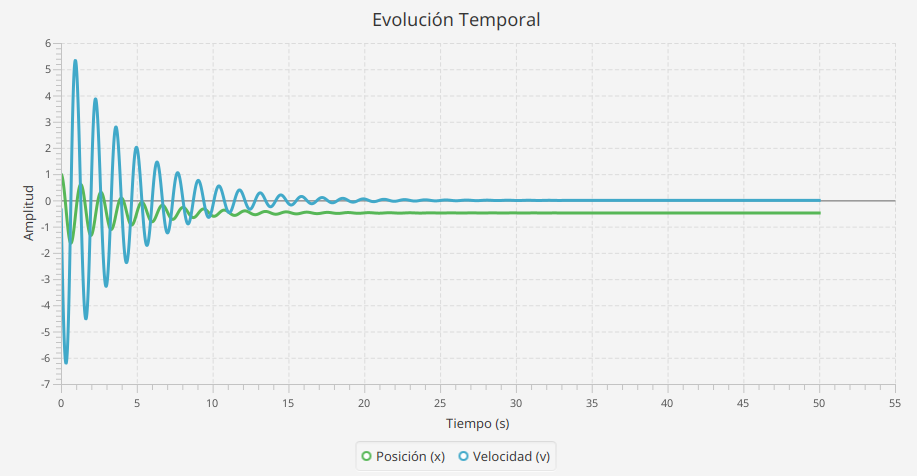
\includegraphics[width=0.7\textwidth]{sist-no-lineal-evol-temp.png}
    }
    \caption{Desplazamiento $x(t)$ y velocidad $v(t)$ en función del tiempo.}
    \label{fig:temporal}
\end{figure}

Y estos son los resultados de la simulación en función de evolución en el tiempo para un sistema lineal.

\begin{figure}[H]
    \centering
    \fbox{
        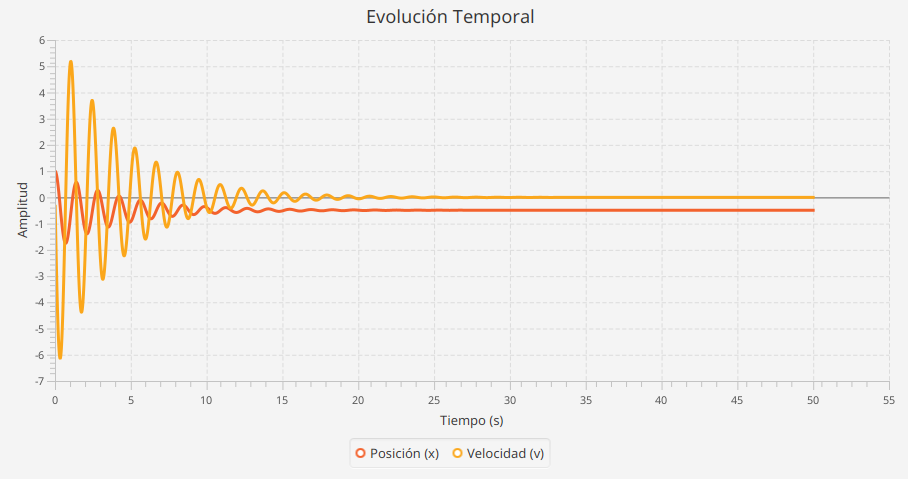
\includegraphics[width=0.7\textwidth]{sist-lineal-evol-temp.png}
    }
    \caption{Desplazamiento $x(t)$ y velocidad $v(t)$ en función del tiempo.}
    \label{fig:temporal}
\end{figure}

\subsection{Diagrama de fase}

Estos son los resultados de la simulación en función del diagrama de fase para un sistema NO lineal.

\begin{figure}[H]
    \centering
    \fbox{
        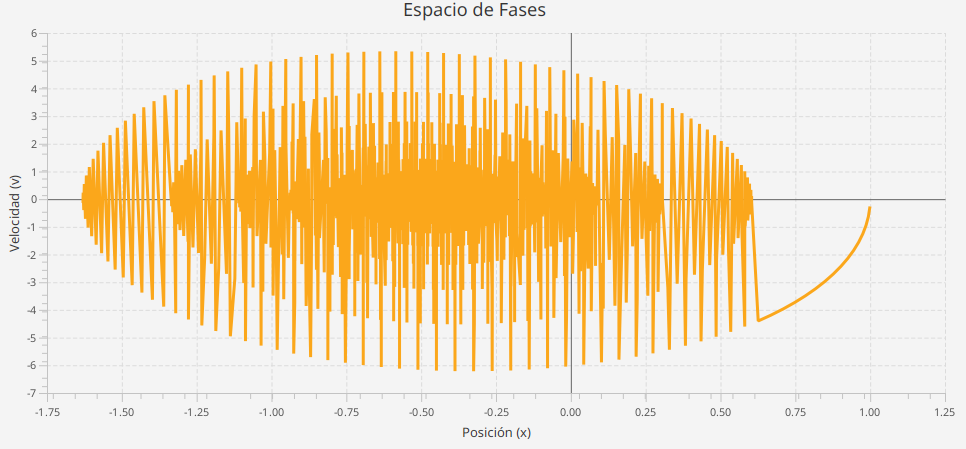
\includegraphics[width=0.7\textwidth]{sist-no-lineal-diag-fase.png}
    }
    \caption{Diagrama de fase $v(t)$ vs.\ $x(t)$.}
    \label{fig:temporal}
\end{figure}

Estos son los resultados de la simulación en función del diagrama de fase para un sistema lineal.

\begin{figure}[H]
    \centering
    \fbox{
        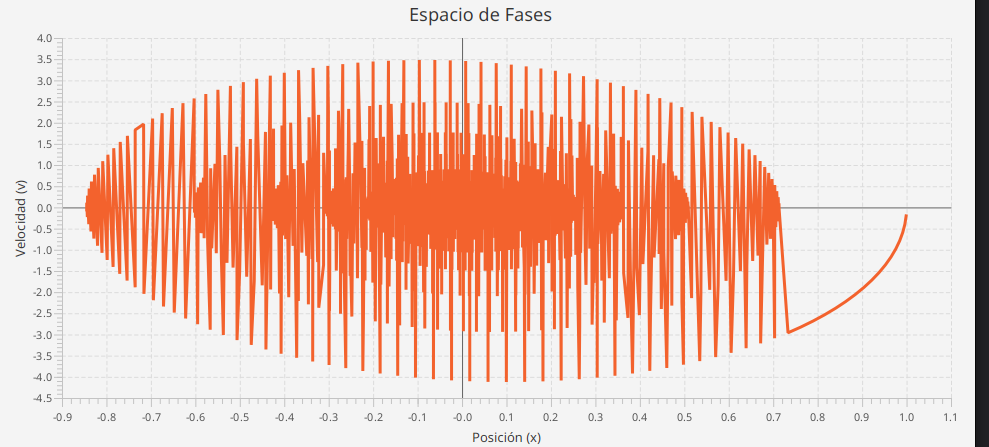
\includegraphics[width=0.7\textwidth]{sist-lineal-diag-fase.png}
    }
    \caption{Diagrama de fase $v(t)$ vs.\ $x(t)$.}
    \label{fig:temporal}
\end{figure}

% ══════════════════════════════════════════════════════════════════════════════
\section{Comparación: sistema lineal vs.\ no lineal}

Podemos observar que el sistema no lineal exhibe una frecuencia de oscilación que varía con la amplitud, mientras que el sistema lineal mantiene una frecuencia constante. Además, el amortiguamiento no lineal hace que el sistema no lineal tarde más en alcanzar el reposo, especialmente cerca del equilibrio, en comparación con el sistema lineal. En el diagrama de fase, el sistema no lineal muestra una trayectoria que se estrecha progresivamente, mientras que el sistema lineal forma una espiral más uniforme hacia el origen.

% ══════════════════════════════════════════════════════════════════════════════
\section{Conclusiones}

En conclusión, la introducción de no linealidades en la rigidez y el amortiguamiento modifica significativamente el comportamiento dinámico del sistema masa-resorte. La frecuencia de oscilación se vuelve dependiente de la amplitud, y el proceso de amortiguamiento se ralentiza cerca del equilibrio. Estas características resaltan la importancia de considerar efectos no lineales en el análisis de sistemas dinámicos reales.

\end{document}